%
% $RCSfile: basic_behaviour.tex,v $
%
% Copyright (C) 2002-2008. Christian Heller.
%
% Permission is granted to copy, distribute and/or modify this document
% under the terms of the GNU Free Documentation License, Version 1.1 or
% any later version published by the Free Software Foundation; with no
% Invariant Sections, with no Front-Cover Texts and with no Back-Cover
% Texts. A copy of the license is included in the section entitled
% "GNU Free Documentation License".
%
% http://www.cybop.net
% - Cybernetics Oriented Programming -
%
% http://www.resmedicinae.org
% - Information in Medicine -
%
% Version: $Revision: 1.1 $ $Date: 2008-08-19 20:41:05 $ $Author: christian $
% Authors: Christian Heller <christian.heller@tuxtax.de>
%

\subsection{Basic Behaviour}
\label{basic_behaviour_heading}
\index{Basic Behaviour in Nature}
\index{A new Kind of Science}
\index{Repetition}
\index{Nesting}
\index{Randomness}
\index{Localised Structures}
\index{Principle of Universality}

Starting from a neutral view to understanding the universe -- and science in
general -- Stephen Wolfram studied the abstract world of rules put into simple
computer programs. \textit{He took the lessons from what kinds of things occur
there and had them in mind when investigating natural systems}, as
\cite{wikipedia} writes. Wolfram's book \emph{A new Kind of Science}
\cite{wolfram} argues that the universe is made up of four basic types of
behaviour (figure \ref{behaviour_figure}):

\begin{enumerate}
    \item \emph{Repetition}
    \item \emph{Nesting}
    \item \emph{Randomness}
    \item \emph{Localised Structures}
\end{enumerate}

\begin{figure}[ht]
    \begin{center}
        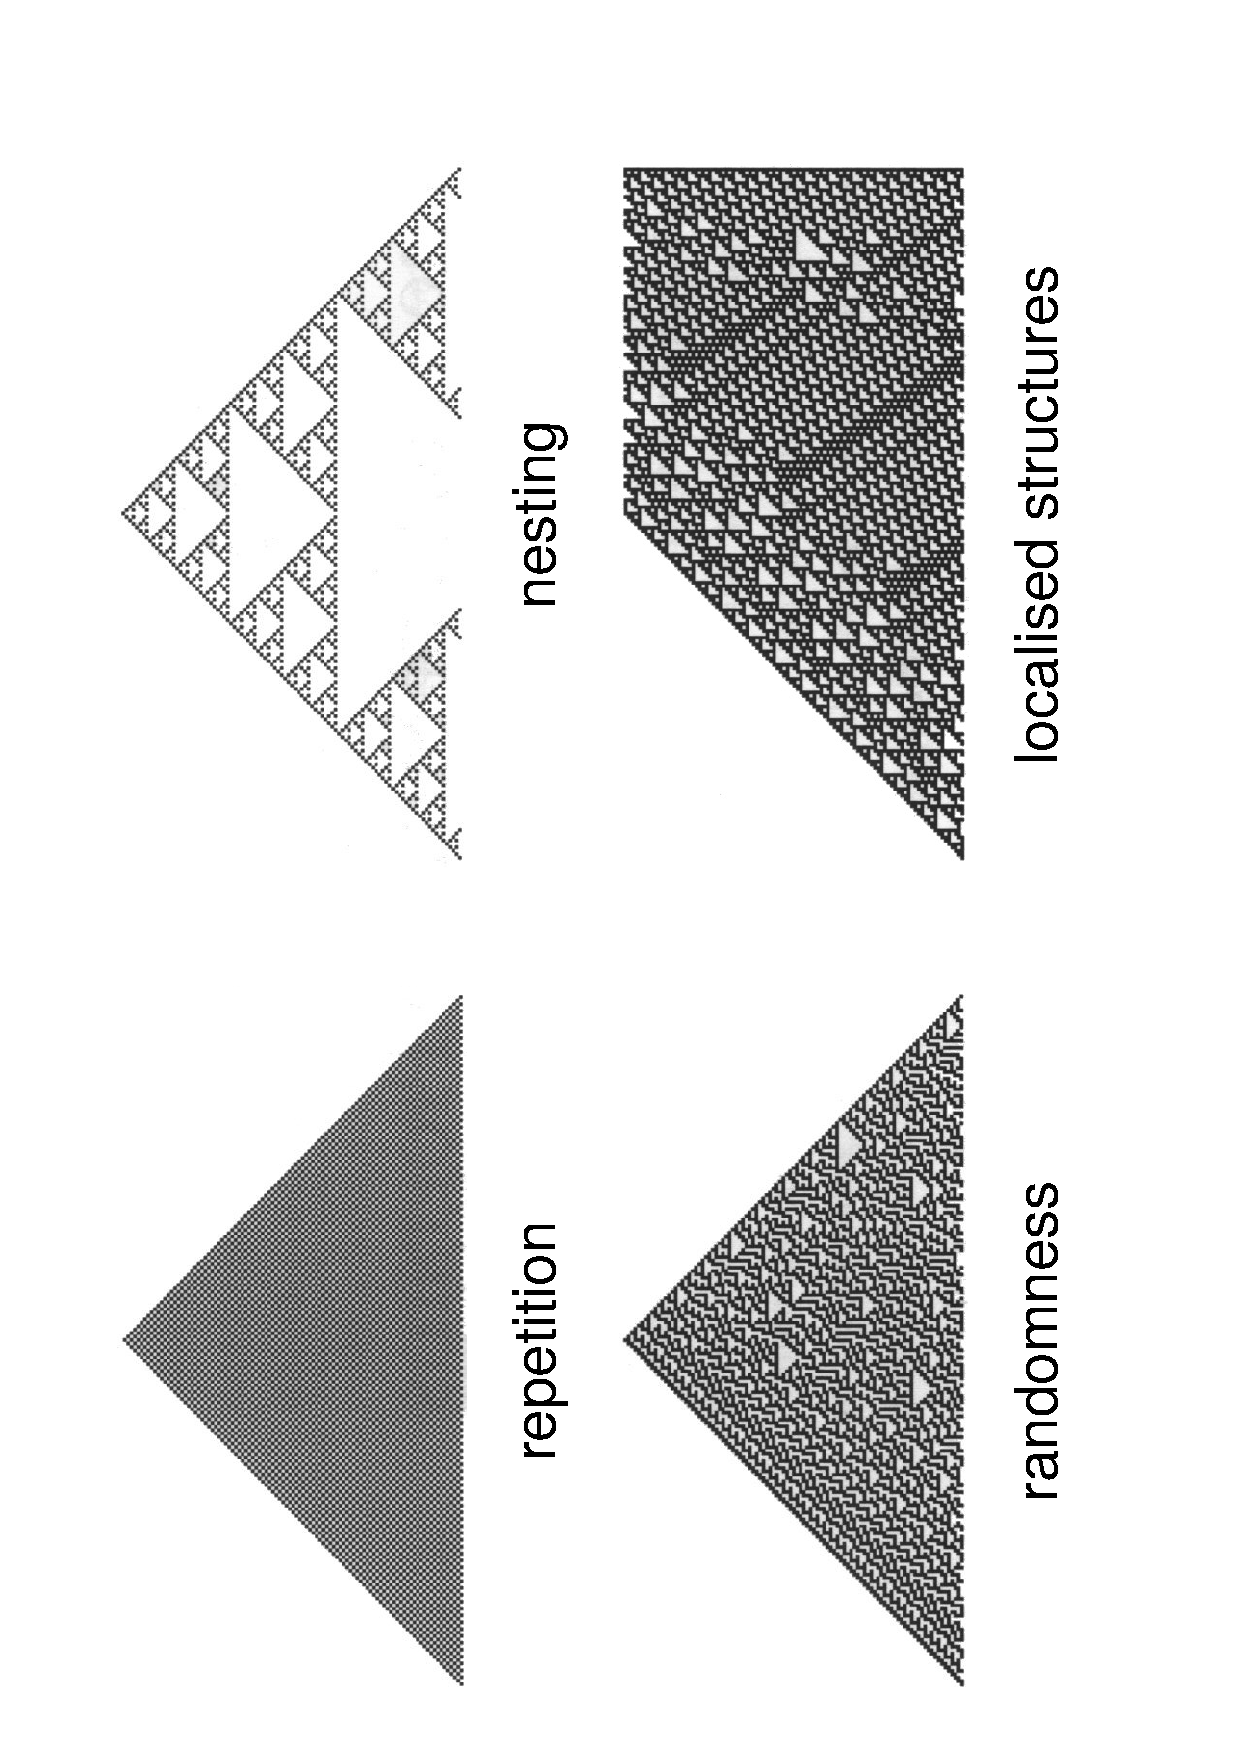
\includegraphics[scale=0.3,angle=-90]{graphic/behaviour.pdf}
        \caption{Wolfram's Four Basic Kinds of Behaviour \cite{wolfram}}
        \label{behaviour_figure}
    \end{center}
\end{figure}

These types of behaviour, after Wolfram, were present everywhere, in nature as
in the whole universe. Just everything in existence contained at least one of
these structures and all sciences were affected by them. Yet while Wolfram
applies results of computing to the study of nature, this work follows the exact
opposite way in that it observes phenomenons of nature and concepts used in
other sciences, and tries to apply them to the design of software systems.
Without knowing a final answer -- the unexpected surprise is that at least two
of Wolfram's findings of basic behaviour match to abstractions as known from
human thinking, and have a pendant in this work:

\newpage

\begin{enumerate}
    \item \emph{Repetition} is the recurrence of equal structures. Yet before
        structures can be compared, they have to be demarcated. This is what
        section \ref{abstraction_heading} will call \emph{Discrimination}
        (later \emph{Itemisation}), and also \emph{Categorisation}.
    \item \emph{Nesting} creates the famous, beautiful \emph{Fractals}. It is
        somewhat similar to \emph{Repetition}, only that the repeated
        structures are not equal in size and do not occur along some chain.
        While the infinity of \emph{Repetition} lies in its neverending
        \emph{Continuation} along some line(s) on the same level, it lies in
        the \emph{Diving} into a deeper level for \emph{Nesting}. Section
        \ref{abstraction_heading} will call this \emph{Composition}.
\end{enumerate}

Wolfram defines a \emph{Principle of Universality} which states that in fact
\emph{all} kinds of systems, even very simple ones, are capable of showing
complex behaviour in form of \emph{Localised Structures}, once some threshold
in the complexity of the underlying rules is passed. But where is this threshold
and who defines what complex behaviour actually is? Does a threshold exist at
all or are the four kinds of behaviour in fact not different? Indeed, one could
argue that neither \emph{Repetition}, nor \emph{Nesting}, nor \emph{Randomness}
are anything special and that it is just the human mind interpreting them as
something special, as assumed by this work. It claims that the human mind gives
structure and meaning to the surrounding real world by building a virtual world.
The principles of human thinking are therefore investigated in the next sections.

Software abstracts human thought which, in order to understand and act in the
surrounding real world, needs to recognise and rely on \emph{known} patterns.
\emph{Randomness} and \emph{Localised Structures} in Wolfram's meaning,
although existent in universe, are rather not used by the human mind to store
information, nor do they seem useful for the design of deterministic software
systems. Of course, information can arrive at- and influence a human mind in an
arbitrary manner and be associated randomly, at will. But the concepts it forms
need to be stable in order to build up knowledge. The research done in this
work therefore relies on reproducible structures making sense to human minds,
namely \emph{Repetition} and \emph{Nesting}.
